%============================== Setting document=============================================

\documentclass[aspectratio=169]{beamer}
\usepackage[italian]{babel} 
\usepackage[utf8]{inputenc} 
\usepackage[T1]{fontenc}
\usepackage{graphicx}
\usepackage{hyperref}
\usepackage{xcolor}
\usepackage{amsmath,amssymb,lmodern}
\usetheme{AnnArbor}
\usepackage{animate}



%change the font localy
\newcommand*{\vet}{\fontfamily{qzc}\selectfont}
% in way to comment a block
\long\def\/*#1*/{}


%==========================Set foot line========================================================
\makeatletter

\setbeamercolor*{author in head/foot}{parent=palette tertiary}
\setbeamercolor*{title in head/foot}{parent=palette primary}
\setbeamercolor*{date in head/foot}{parent=palette primary}

\setbeamercolor*{section in head/foot}{parent=palette tertiary}
\setbeamercolor*{subsection in head/foot}{parent=palette primary}
% colors for the external link field
\setbeamercolor*{LinkToIndex}{parent=palette tertiary}

\defbeamertemplate*{footline}{}
{
	\leavevmode%
	\hbox{%
		\begin{beamercolorbox}[wd=.25\paperwidth,ht=2.25ex,dp=1ex,center]{author in head/foot}%
			\usebeamerfont{author in head/foot}%\insertsection
		\end{beamercolorbox}%
	
		\begin{beamercolorbox}[wd=.25\paperwidth,ht=2.25ex,dp=1ex,center]{title in head/foot}
			%\insertsubsection
		\end{beamercolorbox}%
	
	% this is a new field with an external link
	\begin{beamercolorbox}[wd=.25\paperwidth,ht=2.25ex,dp=1ex,center]{LinkToIndex}%
		\usebeamerfont{author in head/foot}\hyperlink{index}{Indice}\hspace*{2ex}
	\end{beamercolorbox}%

%\usebeamerfont{date in head/foot}\insertshortdate{}\hspace*{2em}
%\insertframenumber{} / \inserttotalframenumber 

		
		\begin{beamercolorbox}[wd=.25\paperwidth,ht=2.25ex,dp=1ex,center]{date in head/foot}%
			\usebeamerfont{date in head/foot}\insertshortdate{}\hspace*{2em}
			\insertframenumber{} / \inserttotalframenumber 
		\end{beamercolorbox}}%
			
	%\usebeamerfont{author in head/foot}\hyperlink{index}{indice}\hspace*{2ex}
		

	\vskip0pt%
}
\setbeamersize{text margin left=1em,text margin right=1em}
\makeatother



\title{Il VHF marino e le procedure di radio telefonia} 
\author{Francesco Rombaldoni\\
Alias Rombo} 
\date{}

\institute{Università degli Studi di Urbino "Carlo Bo"} 
\logo{
\includegraphics[width=15mm]{Imgs/Uni}}

\setbeamercovered{dynamic}

%===========================================Document starting===============================================
\begin{document}
	
	% Cover Page
	\begin{frame} 
		\maketitle 		
	\end{frame}
	
	\section{Premessa}
	\begin{frame}
		\centering{{\textcolor{blue!80}{\huge{\textbf{Premessa}}}}}\\
	\end{frame}

	\begin{frame}{Premessa}
		%\framesubtitle{Parte 1}
		\textbf{L'obiettivo di questa relazione è di esporre il funzionamento, l'utilizzo e la manutenzione degli apparati radio ricetrasmittenti adottati per le radiocomunicazioni in ambito nautico.}\\
		\bigskip
		Per fare ciò la relazione sarà suddivisa in due parti:\\
		\begin{itemize}
			\item La prima parte verterà sulla teoria fisica di base degli apparati radio, al termine della quale si comprenderanno espressioni linguistiche del tipo: \emph{" La maggior parte delle trasmissioni nautiche sono effettuate utilizzando apparati VHF che modulano il segnale in frequenza"}.\\
			\item La seconda parte verterà invece sull'utilizzo e la manutenzione degli impianti ricetrasmittenti di bordo, riservando attenzione alle "buone pratiche" e alle procedure per una comunicazione efficace, al termine della parte si sarà in grado di stabilire una comunicazione con un'altra unità marina o con la capitaneria di porto.
		\end{itemize}
	\end{frame}

	\begin{frame}{Argomenti della relazione}
		%\framesubtitle{Argomenti della prima parte}
		\textbf{Argomenti della prima parte.}
		\begin{itemize}
			\item Proprietà elettromagnetiche della corrente alternata.
			\item Periodo, frequenza, lunghezza e ampiezza d'onda.
			\item Modulazione di ampiezza e Modulazione di frequenza.
			\item Le bande radio.
			\item La radio e l'impianto ricetrasmittente.
		\end{itemize}
	\end{frame}

	\begin{frame}{Argomenti della relazione}
		%\framesubtitle{Argomenti della seconda parte}
		\textbf{Argomenti della seconda parte.}
		\begin{itemize}
			\item La banda nautica.
			\item I canali VHF.
			\item L'alfabeto internazionale. 
			\item La classificazione dei messaggi. 
			\item Trasmissione e ricezione.
		\end{itemize}
	\end{frame}

	\section{Contesto}
	\begin{frame}
		\centering{{\textcolor{blue!80}{\huge{\textbf{Contesto}}}}}\\
	\end{frame}

	\begin{frame}{Contesto}
		\framesubtitle{Introduzione}
		Per trasmettere informazioni, senza disporre di un collegamento fisico tra chi trasmette e chi riceve occorre far transitare su un mezzo non materiale.\\
		\bigskip
		\textbf{Nella trasmissione senza fili il mezzo materiale è costituito da \emph{onde radio}, ovvero da \emph{perturbazioni elettromagnetiche dello spazio}.}\\
		\bigskip
		Le onde radio possono veicolare le informazioni tra una stazione detta \emph{trasmittente} e una stazione detta \emph{ricevente}.\\
	\end{frame}

	\begin{frame}{Contesto}
		\framesubtitle{Come trasmettere informazioni}
			\textbf{Per trasmettere informazioni occorre:}\\
		\begin{itemize}
			\item Generare un'onda radio, detta \emph{onda portante} (quella che veicola le informazioni).
			\item Sovrapporre all'onda portante le informazioni che si desidera veicolare, l'onda che si ottiene è definita \emph{un'onda modulata}.
		\end{itemize} 
		\bigskip
		\textbf{Per ricevere informazioni occorre:}
		\begin{itemize}
			\item Captare l'onda radio trasmessa.
			\item Estrarre dall'onda modulata le informazioni, ovvero \emph{demodulare l'onda}.
		\end{itemize}
	\end{frame}

\section{Proprietà elettromagnetiche della corrente alternata}
\begin{frame}
	\centering{{\textcolor{blue!80}{\huge{\textbf{Proprietà elettromagnetiche della corrente alternata}}}}}\\
\end{frame}
	
\begin{frame}{Introduzione}
	%\framesubtitle{Proprietà elettromagnetiche della corrente alternata}
	Nel 1831 Faraday pubblica un resoconto di una serie di esperimenti nei quali, con modalità opportune, era riuscito a \emph{indurre in un circuito metallico una corrente elettrica} 
	facendo muovere un magnete rispetto al circuito.\\
	\bigskip
	Il fenomeno esaminato da Faraday sarà spiegato nel 1890 dagli studi  sulle interazioni del campo elettrico e del campo magnetico su una carica elettrica svolti da Lorentz; gli studi dimostrano infatti che se una carica elettrica è situata in un campo elettrico e in un campo magnetico sovrapposti, allora su di essa agisce una forza proporzionale: al valore della carica, dalla sua velocità e dall'intensità dei due campi. 
\end{frame}

\begin{frame}{Forza di Lorentz}
	\framesubtitle{Parte 1}
	La forza di Lorentz si ottiene a partire dalla formula per determinare la forza {\vet $\vec{F}$} prodotta da un conduttore di lunghezza {\vet $\vec{l}$} attraversato da una corrente d'intensità {\vet i} e immerso in un campo magnetico uniforme {\vet $\vec{B}$}.\\
	\medskip
	\centering{{\textcolor{red!80}{{\vet$\vec{F}$} = {\vet i $\vec{l}$} X {\vet$\vec{B}$}}}}\\
	\medskip
	\raggedright{Nella quale l'intensità della corrente {\vet i} è considerabile sulla base dell'interpretazione microscopica della corrente:}\\
	\medskip
	\centering{{\vet \textbf{i = e n S v}}}\\
	\medskip
	\raggedright{Dove: {\vet i}  rappresenta l'intensità della corrente, {\vet e} indica il valore assoluto della carica di un elettrone, {\vet n} indica il numero degli elettroni di conduzione contenuti nel conduttore \\ considerato, {\vet S} la sezione del conduttore considerato e {\vet v} la velocità degli elettroni di \\ conduzione presenti nel conduttore.}\\
\end{frame}

\begin{frame}{Forza di Lorentz}
	\framesubtitle{Parte 2}
	Sostituendo l'intesnità della corrente si ottiene:\\  
	\medskip
	\centering{{\textcolor{red!80}{{\vet$\vec{F}$} = {\vet e n S v $\vec{l}$} X {\vet$\vec{B}$}}}}\\
	\medskip
	\raggedright{Tenendo conto del fatto che il vettore {\vet $\vec{l}$} ha la stessa direzione della velocità di deriva {\vet v} e verso opposta ad essa, è possibile considerare la precedente relazione in questo modo:}\\
	\medskip
	\centering{ {{\vet$\vec{F}$}} = -{\vet e n S l $\vec{v}$} X{\vet$\vec{B}$}}\\
	\medskip
	\raggedright{Considerando che il prodotto {\vet S l} corrisponde al volume del conduttore di tratto {\vet l} immerso nel campo magnetico {\vet $\vec{B}$}, ne consegue che il prodotto  {\vet n S l} permette di conoscere il numero {\vet N} di elettroni presente nel conduttore di tratto {\vet l}.\\
	Si può quindi porre:\\}
	\centering{{{\vet$\vec{F}$}} = -{\vet e N $\vec{v}$} X {\vet$\vec{B}$}}\\
\end{frame}

\begin{frame}{Forza di Lorentz}
	\framesubtitle{Parte 3}
	La precedente espressione può essere estesa al caso più generare di una carica (positiva o negativa) di valore assoluto {\vet q} che si muove in un campo magnetico caratterizzato, nel punto dove si trova la carica in un certo istante, dal vettore {\vet $\vec{B}$}.\\
	Ovvero:\\
	\medskip
	\centering{{\textcolor{red!80}{{\vet$\vec{F}$} = {\vet q $\vec{v}$} X {\vet$\vec{B}$}}}}\\
	\medskip
	\raggedright{Siccome non si può escludere che, unitamente al campo magnetico, sia presente anche un campo elettrico {\vet$\vec{E}$}, allora se {\vet$\vec{E}$} indica il vettore del campo elettrico nel punto {\vet P} allora la carica {\vet q} sarà sempre soggetta ad una forza:}\\
	\medskip
	\centering{{\textcolor{red!80}{{\vet$\vec{F}$} = {\vet q $\vec{E}$} + {\vet q $\vec{v}$} X {\vet$\vec{B}$}}}}\\
\end{frame}

\begin{frame}{Corrente indotta dalla forza di Lorentz}
	%\framesubtitle{Proprietà elettromagnetiche della corrente alternata}
La relazione espressa dalla forza di Lorentz consente di prevedere che, quando, con modalità opportune, si muove un circuito (oppure una sua parte) in un campo magnetico, nel circuito si genera una corrente elettrica che non dipende dall'evventuale presenza di un generatore (ad esempio di tipo elettrochimico), per questo motivo la corrente elettrica prodotta è designata con il termine di \textbf{corrente indotta}.\\
\end{frame}

\begin{frame}{Corrente indotta e campo elettromotore}
	\framesubtitle{Parte 1}
	Considerando un \emph{circuito di forma quadrata}, realizzato con un buon conduttore, nel quale sia stato inserito un \emph{amperometro con lo zero centrale}, che sia in movimento (\emph{con velocità costante}) rispetto ad un \emph{campo magnetico uniforme},  in maniera tale che durante il movimento, il circuito entra ed esca dal campo magnetico.\\
	Supponendo che, il circuito si muovi da sinistra verso destra e che il campo magnetico sia posizionato a metà del percorso che il circuito deve compiere, si hanno cinque configurazioni del circuito rispetto al campo magnetico.\\
	\end{frame}

\begin{frame}{Corrente indotta e campo elettromotore}
	\framesubtitle{Parte 2}
	\begin{enumerate}
	\item Il circuito si trova al di fuori del campo magnetico, di conseguenza l'amperometro non indica alcun passaggio di corrente.
	\item Il circuito si trova parzialmente nel campo magnetico, di conseguenza l'amperometro indica la presenza di una corrente d'elettroni che si muove in senso orario. Questa cosa è possibile poiché sugli elettroni di conduzione agisce la forza di Lorentz, di conseguenza si produce una forza elettromotrice data dalla circuitazione del campo elettromotore.
	\item Il circuito si trova completamente immerso nel campo magnetico, di conseguenza nel tratto precedentemente non immerso nel campo magnetico, si  svilupperà un campo elettromotore. Tenendo presente che il fenomeno della corrente indotta è osservabile solo nei circuiti chiusi, è possibile dedurre che il campo elettromotore generato sia\\ opposto a quello della seconda configurazione, facendo in modo che la\\ circuitazione totale valga zero.
\end{enumerate}
	\end{frame}

\begin{frame}{Corrente indotta e campo elettromotore}
	\framesubtitle{Parte 3}
	\begin{enumerate}
		\setcounter{enumi}{3}
		\item Il circuito si trova parzialmente nel campo magnetico, di conseguenza l'amperometro indica la presenza di una corrente d'elettroni che si muove in senso antiorario. 
		\item Il circuito si trova completamente al di fuori del campo magnetico, di conseguenza in esso non sarà più presente alcun campo elettromotore associato alla forza di Lorentz e quindi non sarà percorso da alcuna corrente.
	\end{enumerate}
\end{frame}

\begin{frame}{Legge di Faraday}
	%\framesubtitle{Proprietà elettromagnetiche della corrente alternata}
	L'esperimento precedente oltre permettere di apprezzare l'esistenza della corrente indotta, permette di dimostrare che la genesi del campo elettromotore (il quale poi genera un flusso d'elettroni) è dipendente da una variazione del campo magnetico, infatti quando il circuito dell'esperimento si trovava completamente immerso nel campo magnetico, in esso la somma dei campi elettromotori individuati era nulla.\\
	Il fenomeno appena descritto è interpretabile utilizzando il concetto di flusso del campo magnetico:\\
	\medskip
		\centering{\emph{Quando ad un circuito si concatena una variazione $ \Delta \Phi (\vec{B})$ del flusso del campo magnetico nel tempo $\Delta${\vet t}, nel circuito si produce una corrente indotta determinata dalla presenza di una \textbf{forza elettromotrice} espressa dalla relazione seguente}}\\
	\medskip
	\centering{{\textcolor{red!80}{{\vet fem} = $\frac{\Delta \Phi (\vec{B})}{\Delta t}$}}}\\
	\end{frame}

\begin{frame}{Legge di Faraday-Lenz}
	%\framesubtitle{Proprietà elettromagnetiche della corrente alternata}
	La descrizione della forza elettromotrice indotta espressa dalla legge di Faraday è incompleta, perché in base ad essa non è possibile stabilire il verso di circolazione della corrente indotta.\\
	Faraday aveva dato delle indicazioni chiare sul modo di determinare il verso di circolazione, tuttavia Lenz nel 1834 espose delle osservazioni in grado di semplificare il procedimento proposto da Faraday.\\
	Le osservazioni che Lenz espose sono sintetizzabili in questo modo:\\
	\medskip
	\centering{\emph{La forza elettromotrice indotta in un circuito genera una corrente (detta corrente indotta) il cui effetto deve essere tale da opporsi alla causa che la produce.}}\\
	\medskip
	\raggedright{Per tenere conto della legge di Lenz, la legge di Faraday viene riscritta in questo modo:}\\
	\medskip
	\centering{{\textcolor{red!80}{{\vet fem} = -$\frac{\Delta \Phi (\vec{B})}{\Delta t}$}}}\\
	\end{frame}

\begin{frame}{Corrente autoindotta}
	\framesubtitle{Parte 1}
	Fino a questo momento la legge di Faraday-Lenz è stata usata per interpretare l'effetto che un campo magnetico variabile produce su un circuito chiuso.\\
	Ma un circuito in cui fluisce corrente è un elemento che, a sua volta,  genera un campo magnetico al quale (di conseguenza) si concatena un flusso del campo magnetico.\\
	Se quindi si fa variare l'intensità della corrente che fluisce nel circuito considerato, varierà anche il flusso del campo magnetico che si concatena ad esso. Questa condizione in base alla legge di Faraday-Lenz, determinerà nel circuito stesso la genesi di una corrente indotta.\\
	\medskip
	Trattandosi di corrente indotta dalla variazione dell'intensità della corrente che fluisce nel circuito stesso, essa viene usualmente denominata \textbf{Corrente autoindotta}.\\
	\end{frame}

\begin{frame}{Corrente autoindotta}
	\framesubtitle{Parte 2}
	L'intensità della \textbf{corrente autoindotta} è determinata dal valore della variazione nel tempo del flusso che si concatena al circuito. Ricordando che il valore del flusso autoconcatenato dipende a sua volta dalle caratteristiche geometriche del circuito e dalle caratteristiche del mezzo con cui il circuito è realizzato.\\
	\medskip
	\centering{\emph{In generale, ad ogni circuito è possibile associare una grandezza, denominata \textbf{coefficiente di autoindizione} (detto anche induttanza) che si indica con il simbolo{\vet L}, che connette il valore dell'intensità di corrente che fluisce nel circuito con il valore $\Phi(\vec{B})$ del flusso del campo magnetico autoconcatenato, secondo la relazione:}}\\
	\medskip
	\centering{{\textcolor{red!80}{$\Phi(\vec{B})$ = {\vet L i}}}}
\end{frame}

\begin{frame}{Radiazione elettromagnetica}
	\framesubtitle{Parte 1}
	In generale, nella realtà, un flusso variabile di $\vec{B}$ (o di $\vec{E}$) non genera un campo $\vec{E}$ (o un campo $\vec{B}$) anch'esso variabile; tuttavia in opportune condizioni ciò può accadere.\\
	\medskip
	Se $\vec{B}$ variasse sinusoidalmente secondo l'ecquazione:\\ 
	\smallskip
	{\textcolor{black!50}{${\vet B} = C_{1} \sin (\omega {\vet t})$}}\\
	\smallskip
	Il campo elettromotore associato alla variazione del flusso di $\vec{B}$ rispetto al tempo sarebbe del tipo:\\
	\smallskip
	{\textcolor{black!50}{${\vet E} = C_{2} \cos (\omega {\vet t})$}}\\
	\smallskip
	D'altra parte, ad un campo elettrico di questo tipo, è associato un flusso la cui variazione rispetto al tempo genererà un campo $\vec{B}$ del tipo:\\
	\smallskip
	{\textcolor{black!50}{${\vet B} = C_{3} \sin (\omega {\vet t})$}}
 	\end{frame}
 
 \begin{frame}{Radiazione elettromagnetica}
 	\framesubtitle{Parte 2}
 	Per cui si deduce che:\\
 	\medskip
 	\centering{\emph{Un campo magnetico variabile in modo opportuno concatena a sè un campo elettromotore, variabile in modo tale da concatenare a se un campo magnetico variabile... e così via.\\ In questo caso, i campi elettrico e magnetico concatenati costituiscono un ente fisico, solitamente indicato con il termine di \textbf{radiazione elettromagnetica}}}\\
 	\medskip
 	%\animategraphics[loop,width=4cm]{10}{GifImages/Wavey/Wavey-}{0}{30}
 	%\caption{{\textcolor{gray!80}{[Immagine animata]}}}
 	%\raggedright
		\begin{figure}
			\begin{columns}
				\hfill
				\column{.1\linewidth}
				\animategraphics[loop,width=3\textwidth]{10}{GifImages/Wavey/Wavey-}{0}{30}
				\column{.3\linewidth}
				%\caption{{\textcolor{gray!80}{[Immagine animata]}}}
			\qquad \tiny{\textcolor{gray!80}{[Immagine animata]}}
			\end{columns}
		\end{figure}
		
 	
 \end{frame}

\begin{frame}{Propagazione della radiazione elettromagnetica}
	\framesubtitle{Parte 1}
	In un generico punto distante {\vet x} dall'origine del sistema di riferimento, e nel generico istante {\vet t}, i valori di $\vec{E}$ e di $\vec{B}$ sono dati da:\\
	\medskip
	\centering{{\textcolor{red!80}{$E = E_{0} \sin [2 \pi (\frac{t}{T} - \frac{x}{\lambda})]$}}}\\
	\smallskip
	{\textcolor{red!80}{$ B = B_{0} \sin [2 \pi (\frac{t}{T} - \frac{x}{\lambda})]$}}\\
	\raggedright
	\medskip
	Dove: $\lambda$ indica la lunghezza d'onda della radiazione elettromagnetica e T indica il periodo.\\
	\medskip
	Come precedentemente osservato, i vettori $\vec{E}$ e $\vec{B}$ che caratterizzano una radiazione elettromagnetica, giacciono in piani perpendicolari fra loro, possedendo una direzione di vibrazione perpendicolare alla direzione di propagazione. Questa rappresentazione corrisponde al fatto che una radiazione elettromagnetica che si propaga nello spazio si comporta\\ come \emph{un'onda trasversale}.
\end{frame}

\begin{frame}{Propagazione della radiazione elettromagnetica}
	\framesubtitle{Parte 2}
	I moduli di $\vec{E}$ e $\vec{B}$ variano in funzione dell'intensità della radiazione, della distanza {\vet x} del punto considerato dalla sorgente e del tempo {\vet t}; tuttavia si può dimostrare che essi stanno fra loro sempre nel rapporto seguente:\\
	\medskip
	\centering{{\textcolor{red!80}{{\vet v} = $\frac{E}{B}$}}}\\
	\medskip
	\raggedright{dove {\vet v} indica la velocità di propagazione della radiazione.}\\
\end{frame}

\begin{frame}{Generazione delle radiazioni elettromagnetiche}
	\framesubtitle{Parte 1}
	La prima persona ad aver svolto esperimenti per lo studio della radiazione elettromagnetica è stato il fisico tedesco Hertz, che, nel 1882 fu in grado di generare radiazioni elettromagnetiche.\\
	L'apparecchiatura utilizzata da Hertz per studiare le radiazioni elettromagnetiche si può considerare come un trasformatore di differenza di potenziale, che tra due elettrodi produce una differenza di potenziale molto elevata, capace di provocare una scarica elettrica.\\ 
	\medskip
	Per verificare quindi l'ipotesi di propagazione del campo elettromagnetico, Hertz posizionò nelle vicinanze del generatore un secondo circuito con caratteristiche de tutto simili al primo, osservando se in questo secondo circuito (detto rilevatore) si manifestava un qualche effetto fisico dovuto alla scarica provocata dal generatore. Constatando che ogni qualvolta venisse prodotta una scarica fra gli elettrodi del generatore, veniva indotta una scarica\\ tra gli elettrodi del rilevatore.\\
\end{frame}

\begin{frame}{Generazione delle radiazioni elettromagnetiche}
	\framesubtitle{Parte 2}
	Il generatore di Hertz non è molto adatto come generatore di radiazioni elettromagnetiche, perché il circuito assorbe una grande quantità di energia. Una progressiva modifica del generatore di Hertz ha portato alle moderne \textbf{antenne ricetrasmittenti}.\\
	\medskip
	In esse, gruppi di cariche di segno opposto oscillano con moto armonico, generando intensi campi elettromagnetici.\\
	L'estrema schematizzazione di un'antenna è costituita da un \textbf{dipolo elettrico oscillante}.\\
	\medskip
	\centering{\emph{Si può dimostrare che a grandi distanze dal dipolo il campo elettrico $\vec{E}$ si trova sempre in piani passanti per il dipolo, e la sua intensità: è inversamente proporzionale alla distanza {\vet r} dal dipolo, è direttamente proporzionale al quadrato della frequenza {\vet f} di oscillazione del dipolo e dipende dall'angolo $\vartheta$ che la direzione considerata forma con l'asse del dipolo.}}\\
	\medskip
	\raggedright{Ricordando che l'intensità si un'onda è proporzionale al quadrato della sua ampiezza, si\\ ottiene la formula:}\\
	\centering{{\textcolor{red!80}{$I \div E^2 \div \frac{f^4 \sin^2 \vartheta}{r^2}$}}}
\end{frame}

\begin{frame}{Energia della radiazione elettromagnetica}
	\framesubtitle{Parte 1}
	A partire dal caso di un campo elettrico uniforme confinato tra due armature di un condensatore piano, è possibile determinare che un campo elettrico è sede di energia, la cui densità è data dalla seguente relazione:\\
	\smallskip
	\centering{$D_{E} = \frac{1}{2} \varepsilon_{0} E^2$}\\
	\smallskip
	\raggedright{Analogamente l'analisi di un particolare campo magnetico uniforme (come quello prodotto all'interno di un solenoide) consente di stabilire che anche un campo magnetico è sede di energia, la cui densità è data dalla relazione:}\\
	\smallskip
	\centering{$D_{B} = \frac{1}{2} \frac{B^2}{\mu_{0}}$}\\
	\smallskip
	\raggedright{La densità di energia $D_{E,B}$ associata al campo elettromagnetico della radiazione, quando i moduli dei campi sono $E$ e $B$ rispettivamente è allora data da:}\\
	\smallskip
	\centering{$D_{E,B} = D_{E} + D_{B} = \frac{1}{2} \varepsilon_{0} E^2 + \frac{1}{2} \frac{B^2}{\mu_{0}}$}
\end{frame}

\begin{frame}{Energia della radiazione elettromagnetica}
	\framesubtitle{Parte 2}
	I valori di {\vet E} e di {\vet B} che compaiono nella precedente relazione sono funzione del tempo {\vet t}\\
	\medskip
	\centering{$E = E_{max} \sin \omega t \qquad B = B_{max} \sin \omega t$}\\ 
	\medskip
	\raggedright{Per calcolare l'energia di una radiazione che attraversa una certa superficie, si deve perciò determinare il valore medio dell'espressione precedente, valutata su un periodo {\vet T} della radiazione. Con il calcolo integrale si trovano i seguenti valori medi:}\\
	\medskip
	\centering{$\frac{1}{4} \varepsilon_{0} E^2_{max} \quad \textrm{e} \quad \frac{1}{4} \frac{B^2_{max}}{\mu_{0}}$}\\
	\medskip
	\raggedright{Ricordando poi che $E_{max} = c B_{max}$ e che $c^2 = 1/(\varepsilon_{0} \mu_{0})$, si ottiene infine:}\\
	\medskip
	\centering{{\textcolor{red!80}{$\frac{\varepsilon_{0} E^2_{max}}{4} + \frac{E^2_{max}}{4c^2\mu_{0}} = \frac{\varepsilon_{0} E^2_{max}}{2}
				\qquad \frac{\varepsilon_{0} c^2 B^2_{max}}{4} + \frac{B^2_{max}}{4\mu_{0}} = \frac{B^2_{max}}{2\mu_{0}}$}}}
\end{frame}

\begin{frame}{Energia della radiazione elettromagnetica}
	\framesubtitle{Parte 3}
	Queste relazioni consentono di determinare l'energia elettromagnetica che attraversa l'unità di superficie nell'unità di tempo, ovvero la potenza della radiazione per unità di superficie, detta anche \textbf{potenza specifica} o \textbf{irraggiamento}.\\
	Tenendo conto, infatti che tale energia è quella che si può pensare contenuta in un cilindro di altezza $(c \cdot 1 s)$ e di base $1 m^2$, ottenendo: \\
	\medskip
	\centering{{\textcolor{red!80}{$I = \frac{1}{2} c \varepsilon_{0} E^2_{max} = \frac{1}{2} c \frac{B^2_{max}}{\mu_{0}}$}}}
\end{frame}

\section{Periodo, frequenza, lunghezza e ampiezza d'onda}
\begin{frame}
	\centering{{\textcolor{blue!80}{\huge{\textbf{Periodo, frequenza, lunghezza e ampiezza d'onda}}}}}\\
\end{frame}

\begin{frame}{Periodo e frequenza}
	%\framesubtitle{Periodo, frequenza, lunghezza e ampiezza d'onda}
	In fisica la frequenza di un fenomeno che si ripete identico nel tempo, viene data dal numero di ricorrenze dell'evento in una data unità di tempo.\\
	\smallskip
	Un modo per calcolare il valore della \textbf{frequenza} ({\vet f}) consiste nel fissare un intervallo di tempo chiamato \textbf{periodo} (T), nel contare il numero delle occorrenze dell'evento che si ripete nell'intervallo di tempo considerato e nel dividere quindi il risultato di questo conteggio per il periodo.\\
	In formula:\\
	\medskip
	\centering{{\textcolor{red!80}{{\vet f} = $\frac{1}{T}$}}}\\
	\medskip
	\raggedright{L'unità di misura della frequenza è chiamata \textbf{hertz} (Hz), dove 1Hz caratterizza un evento che occorre una volta in un secondo.}\\
	Quindi:\\
	\centering{1Hz = $\frac{1}{s}$}
\end{frame}

\begin{frame}{Lunghezza e ampiezza d'onda}
	\framesubtitle{Parte 1}
	\emph{Un'onda è una struttura ripetitiva tanto nello spazio che nel tempo.}\\
	\smallskip
	La \textbf{lunghezza d'onda} di un'onda periodica è la distanza tra due massimi o fra due minimi, e viene comunemente indicata con $\lambda$.\\
	\centering
	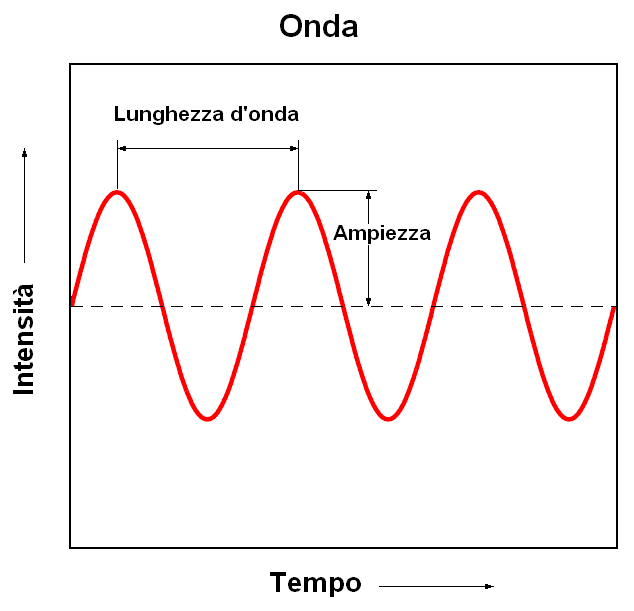
\includegraphics[width=0.3\textwidth]{Imgs/Onda}
\end{frame}

\begin{frame}{Lunghezza e ampiezza d'onda}
	\framesubtitle{Parte 2}
	La lunghezza d'onda $\lambda$ è definita come:\\
	\medskip
	\centering{$\lambda = \frac{{\vet v}}{{\vet f}}$}\\
	\smallskip
	\raggedright{Dove {\vet v} è la velocità di propagazione e {\vet f} la frequenza dell'onda. La velocità {\vet v} delle onde elettromagnetiche è pari alla velocità della luce (circa $3 \cdot 10^8 m\mathbin{/}s$)}.\\
	\medskip
	Per esempio, la lunghezza d'onda $\lambda$ di un segnale a 100MHz (quindi il segnale di un'onda radio) è circa:\\
	\medskip
	\centering{$\frac{3 \cdot 10^8 m\mathbin{/}s}{100 \cdot 10^6 Mh} = 3m$}\\
	\medskip
	\raggedright{In sintesi:}\\
	\emph{La \textbf{lunghezza d'onda} che viene misurata in metri, rappresenta la distanza tra i massimi \\ed i minimi dell'onda. Mentre il valore della sua \textbf{ampiezza} consiste nella distanza che intercorre tra il suo massimo ed il suo valore nullo.}
\end{frame}

\begin{frame}{Relazione tra lunghezza d'onda e frequenza}
	Le onde radio sono quindi delle \textbf{perturbazioni elettromagnetiche nello spazio} caratterizzate da una \textbf{lunghezza d'onda} e da una frequenza.\\
	Poiché la lunghezza d'onda e la frequenza di una radiazione sono \textbf{inversamente proporzionali}, tanto minore sarà la lunghezza d'onda, tanto maggiore sarà la frequenza.\\
	\medskip
	Per esempio:\\
	\centering
	\begin{tabular}{|c|c|c|}
		\hline
		\textbf{Banda}& \textbf{Frequenza} & \textbf{Lambda} \\
		\hline
		OM (radioamatori)& 14Mhz & 21m \\
		\hline
		CB (banda cittadina)& 27Mhz & 11m\\
		\hline
		AG (aviazione)& 118Mhz & 2,54m \\
		\hline
		Nautica VHF (marittima)& 156Mhz & 1.92m \\
		\hline
	\end{tabular}
\end{frame}

\section{Modulazione di ampiezza e Modulazione di frequenza}
\begin{frame}
	\centering{{\textcolor{blue!80}{\huge{\textbf{Modulazione d'ampiezza e Modulazione di frequenza}}}}}\\
\end{frame}

\begin{frame}{Modulazione di ampiezza}
	\framesubtitle{Introduzione}
	In telecomunicazioni, la \textbf{modulazione di ampiezza} (sigla \textbf{AM}), è una tecnica di trasmissione usata per trasmettere informazioni. La quale consiste nel modulare l'ampiezza del segnale radio che s'intende utilizzare per la trasmissione (detto \textbf{segnale portante}), in maniera proporzionale all'ampiezza del segnale che s'intende trasmettere (detto \textbf{segnale modulante}) che contiene l'informazione.\\
	\medskip
	La modulazione di ampiezza è molto semplice da realizzare, per questo motivo è stata utilizzata agli albori delle trasmissioni radio.\\
	\medskip
	I principali inconvenienti legati all'utilizzo di questa tecnica sono: l'estrema sensibilità ai disturbi e alle condizioni di propagazione, in quanto qualsiasi disturbo, nonché le \\ variazioni aleatorie dell'attenuazione offerte dal mezzo trasmissivo durante la \\propagazione.
\end{frame}


\begin{frame}{Modulazione di ampiezza}
	\framesubtitle{Descrizione}
	
	\begin{columns}
		% Column 1
		\begin{column}{0.6\textwidth}
			Supponendo di utilizzare come \textbf{onda portante} (di frequenza maggiore rispetto all'onda modulante), un'onda periodica in questa forma:\\
			\smallskip
			\centering{{\textcolor{red!80}{$v_{p}(t) = V_{p}\cos(\omega_{p}t)$}}\qquad (Prima figura)}\\
			\smallskip
			\raggedright{E come \textbf{onda modulante}, un'onda periodica in questa forma:}\\
			\smallskip
			\centering{{\textcolor{red!80}{$v_{m}(t) = V_{m}\cos(\omega_{m}t)$}} \qquad(Seconda figura)}\\
			\smallskip
			\raggedright{Ricordando che pulsazione, frequenza e periodo sono legate fra loro:}\\
			\smallskip
			\centering{{\vet f} = $\frac{1}{T}$\quad$\omega = 2 \pi$ {\vet f} = $\frac{2\pi}{T}$}\\
			\smallskip
			\raggedright{Pertanto il segnale modulato dovrà risultare:}\\
			\smallskip
			\centering{{\textcolor{red!80}{$v_{am}(t) = (V_{p} + V_{m} \cos(\omega_{m}t))\cos(\omega_{p}t)$}} \quad (Terza figura)}\\
		\end{column}
		% Column 2    
		\begin{column}{0.4\textwidth}
			\begin{figure}
			%	\centering
			\raggedright
			%\hfill
			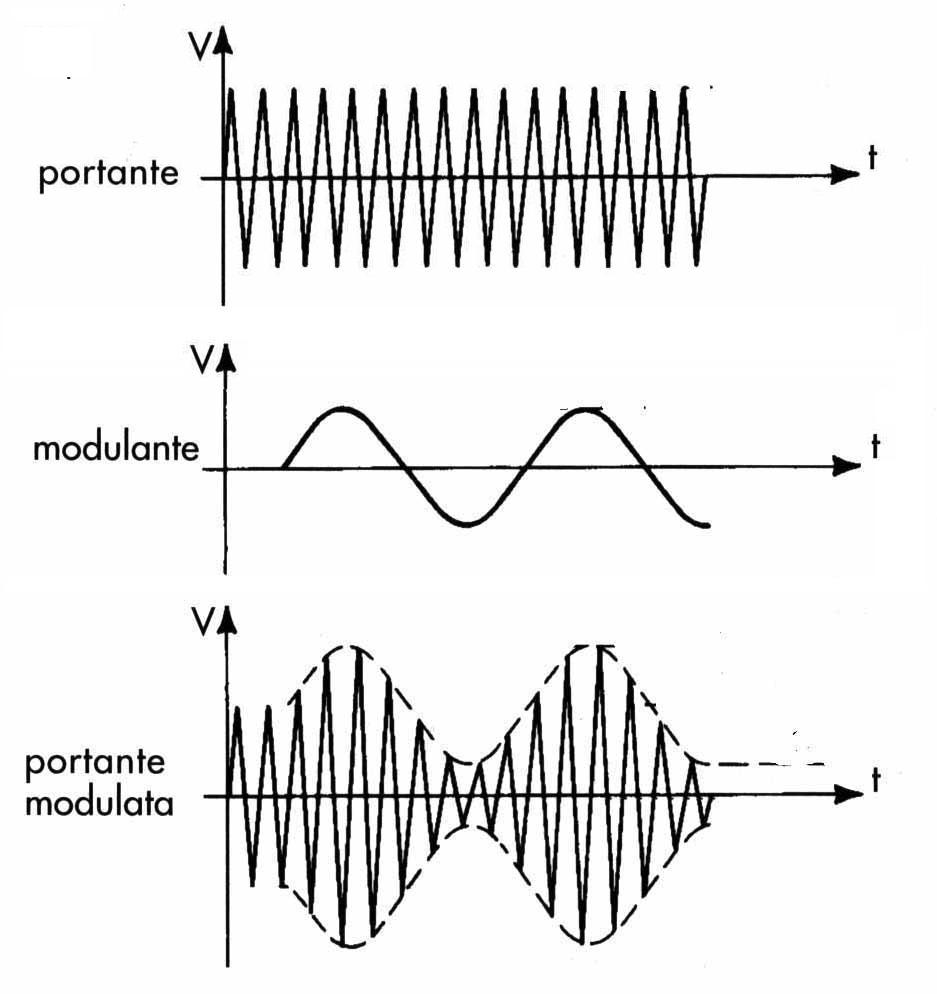
\includegraphics[width=0.8\textwidth]{Imgs/Modulante}
			\end{figure}
		\end{column}
	\end{columns}
	\end{frame}

\begin{frame}{Modulazione di frequenza}
	\framesubtitle{Introduzione}
	La \textbf{modulazione di frequenza} (sigla \textbf{FM}), nelle telecomunicazioni è una delle tecniche di trasmissione utilizzate per trasmettere informazioni.\\
	Consiste nel modulare la frequenza del segnale radio che s'intende utilizzare per la trasmissione (detto portante) in maniera proporzionale all'ampiezza del segnale che s'intende trasmettere.\\
	\medskip
	Rispetto alla \textbf{modulazione di ampiezza}, possiede il vantaggio di essere molto meno sensibile ai disturbi e permette una trasmissione di maggiore qualità. Possiede inoltre una efficienza energetica molto superiore, in quanto la potenza del segnale modulato FM è esclusivamente quella della portante. (Il segnale della informazione, non richiede potenza aggiuntiva per poter essere trasmesso).\\
	\medskip
	Il difetto principale è la necessità di circuiti molto più complessi, sia per la trasmissione\\ che per ricezione  del segnale, nonché, una maggiore richiesta di banda in trasmissione. \\
	\end{frame}

\begin{frame}{Modulazione di frequenza}
	\framesubtitle{Descrizione parte 1}
	Supponendo di utilizzare come \textbf{onda portante} un'onda periodica in questa forma:\\
	\smallskip
	\centering{{\textcolor{red!80}{$v_{p}(t) = V_{p}\cos(\omega_{p}t)$}}}\\
	\smallskip
	\raggedright{E come \textbf{onda modulante}, un'onda periodica in questa forma:}\\
	\smallskip
	\centering{{\textcolor{red!80}{$v_{m}(t) = V_{m}\cos(\omega_{m}t)$}}}\\
	\smallskip
	\raggedright{Dove: $\omega_{p}>>\omega_{m}$}\\
	\smallskip
	\raggedright{Mentre nel segnale della portante la pulsazione $\omega_{p}$ possiede valore costante, la pulsazione del segnale modulato deve essere proporzionale, secondo una costante $K_f$ caratteristica del modulatore, all'ampiezza del segnale modulante}\\
	\smallskip
	Per cui la pulsazione istantanea del segnale modulato in \textbf{FM} deve avere la forma:\\
	\quad \textcolor{red!80}{$\omega_{FM}(t) $} $= \omega_{p} + K_{f} V_{m} \cos(\omega_{m}t)$
	$= 2\pi(f_{p} + \frac{K_{f} V_{m}}{2\pi} \cos(\omega_{m}t))$
	\textcolor{red!80}{$= 2\pi(f_{p} + \Delta f \cos(\omega_{m}t))$}\\
	\smallskip
	\raggedright{Dove: $\Delta f = \frac{K_{f} V_{m}}{2\pi}$ indica lo spostamento massimo di frequenza rispetto al valore $f_{p}$ \\della portante}
\end{frame}


\begin{frame}{Modulazione di frequenza}
	\framesubtitle{Descrizione parte 2}
	
		\begin{columns}
		% Column 1
		\begin{column}{0.6\textwidth}
			La pulsazione istantanea e l'angolo istantaneo sono legati dalla relazione:\\
			%\smallskip
			\centering{$\omega(t) = \frac{d\varphi(t)}{dt}$}\\
			%\smallskip
			\raggedright{Per cui:}\\
			%\smallskip
			\centering{$d\varphi(t) = \omega(t)dt$}\\
			\smallskip
			\raggedright{Dalla quale integrando si ottiene:}\\
			\smallskip
			\centering
			\textcolor{red!80}{$\varphi(t) = $} $\int(\omega_{p} K_{f} V_{m} \cos(\omega_{m}t))dt =$\\
			\smallskip
			$=$ \textcolor{red!80}{$\omega_{p}t + \frac{K_{f} V_{m}}{\omega_{m}} \sin(\omega_{m}t)$}\\
			\smallskip
			\raggedright{Ora è possibile trovare il valore del segnale modulato:}\\
			\smallskip
			\centering
			\textcolor{red!80}{$v_{FM}(t) = $} $V_{p} \cos(\omega_{p}t+\frac{K_{f} V_{m}}{\omega_{m}}\sin(\omega_{m}t)) =$\\
			\smallskip
			$=$ \textcolor{red!80}{$V_{p}\cos(\omega_{p}t + m\sin(\omega_{m}t))$}\\
			\smallskip
			\raggedright{Dove: $m = \frac{K_{f} V_{m}}{\omega_{m}} = \frac{K_{f} V_{m}}{2\pi f_{m}} = \frac{\varDelta f}{f_{m}}$ indica l'indice di modulazione in frequenza}
			
		\end{column}
		% Column 2    
		\begin{column}{0.4\textwidth}
			\begin{figure}
				%	\centering
				\raggedright
				%\hfill
				\animategraphics[loop,width=0.8\textwidth]{10}{GifImages/FM/FM-}{0}{31}\\
				\qquad \qquad \tiny {\textcolor{gray!80}{[Immagine animata]}}
			\end{figure}
		\end{column}
	\end{columns}
	
\end{frame}

\section{Le bande radio}
\begin{frame}
	\centering{{\textcolor{blue!80}{\huge{\textbf{Le bande radio}}}}}\\
\end{frame}

\begin{frame}{Introduzione}
	Nelle telecomunicazione con il termine \textbf{banda radio} (o \textbf{spettro radio}) si indica la sezione dello spettro elettromagnetico utilizzata per la radio-trasmissione di dati e informazioni.\\
	Il termine banda radio identifica la suddivisione spettrale del mezzo trasmissivo, ripartita in modo che più utenti e operatori possano utilizzare il mezzo trasmissivo evitando interferenze oppure conflitti di utilizzazione.\\
	\medskip
	%Le bande sono soggette ad un piano di \emph{attribuzione} delle frequenze in base alla destinazione di un servizio di radiocomunicazione, con successiva \emph{assegnazione} ad un operatore oppure una \emph{allocazione} geografica su un territorio.\\
	L'obbiettivo è quello di ottimizzare l'uso dello spettro radio evitando le interferenze tra i servizi, Per questo motivo l'assegnazione delle frequenze avviene tipicamente attraverso tecniche di tipo "\textbf{Frequency Division Multiplexing}" (FDM).\\
	Questo tipo di assegnazione implica tipicamente la presenza di adeguate bande di guardia la le varia bande attribuite/assegnate/allocate, appunto per evitare la reciproca interferenza.
\end{frame}

\begin{frame}{Frequency Division Multiplexing}
	\framesubtitle{Definizione}
	In telecomunicazioni la \textbf{Multiplazione a Divisione di Frequenza}, conosciuta anche come \textbf{FDM} (acronimo inglese di \textbf{Frequency Division Multiplexing}) è una tecnica di condivisione di un canale di trasmissione secondo la quale l'intero canale disponibile viene diviso in \textbf{sottocanali}, ognuno costituito da una \textbf{sottobanda} di frequenze e separato da un altro grazie ad un piccolo intervallo di guardia. I diversi sottocanali sono quindi assegnati a diverse sorgenti trasmissive e a diversi utenti, i quali dunque possono così comunicare contemporaneamente sullo stesso canale senza incorrere nella mutua interferenza. \\
	\smallskip
	Questa tecnica può essere utilizzata solo nel caso di trasmissione di segnali analogici, per tanto è soggetta ai problemi di distorsione e rumore di fondo.\\
	\end{frame}

\begin{frame}{Frequency Division Multiplexing}
	\framesubtitle{Esempio}
	La figura seguente mostra un esempio di FDM in cui tre segnali S1, S2, S3 con banda limitata fra 0 e 4 kHz vengono trasmessi su un unico canale. Ad ogni segnale viene assegnata una porzione di banda di 4 kHz dell'intero canale, per mezzo di una traslazione in frequenza della banda del segnale stesso. In ricezione quindi i diversi segnali vengono estratti dal canale e separati.\\
	\smallskip
	\centering
		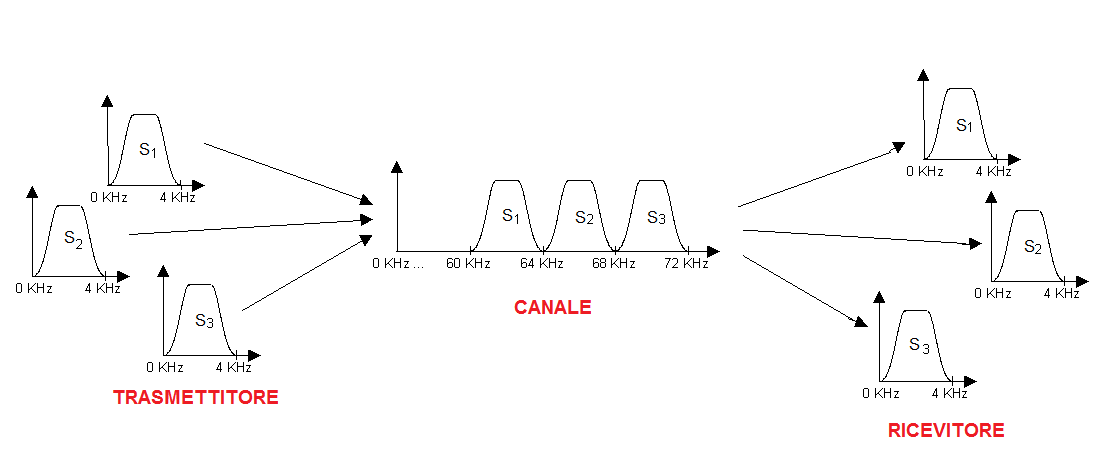
\includegraphics[width=0.6\textwidth]{Imgs/FDM}
	\end{frame}

\begin{frame}{Attribuzione generale delle frequenze}
	\resizebox{\textwidth}{!}{
	\begin{tabular}{|c|c|c|c|c|}
		\hline
		\textbf{Denominazione ITU}&\textbf{Banda}  &\textbf{Frequenze}  &\textbf{Lunghezza d'onda}  &\textbf{Utilizzo più comune}  \\
		\hline
		Extremely Low Frequency& \textbf{ELF} & 3 - 30 Hz & 100 000 - 10 000 km & Radioastronomia - Telerilevamento - satelliti meteo  \\
		\hline
		Super Low Frequency& \textbf{SLF} & 30 - 300 Hz & 10 000 - 1000 km  & Comunicazioni subacquee - analisi elettromagnetiche e geofisiche \\
		\hline
		Ultra Low Frequency & \textbf{ULF} & 300 - 3000 Hz & 1000 - 100 km & Comunicazioni subacquee - analisi elettromagnetiche e geofisiche \\
		\hline
		Very Low Frequency& \textbf{VLF} & 3 - 30 kHz & 100 - 10 km & Comunicazioni subacquee - analisi elettromagnetiche e geofisiche \\
		\hline
		Low Frequency& \textbf{LF} & 30 - 300 kHz & 10 - 1 km & Radiofari aeronautici - navigazione marittima - informazioni e sistemi meteorologi\\
		\hline
		Medium Frequency& \textbf{MF} & 300 - 3000 kHz & 1000 - 100 m  & Broadcast\\
		\hline
		High Frequency& \textbf{HF} &3 - 30 MHz  & 100 - 10 m   & Radiodiffuzione a lunga distanza - radioamatori\\
		\hline
		Very High Frequency& \textbf{VHF} & 30 - 300 MHz & 10 - 1 m  & Aviazione generale - unità navali - forze di polizie - canali televisivi\\
		\hline
		Ultra High Frequency& \textbf{UHF} & 300 - 3000 MHz & 100 - 10 cm  & Canali televisivi - telefonia cellulare, reti wireless - aeronautiche militari\\
		\hline
		Super High Frequency& \textbf{SHF} & 3 - 30 GHz & 10 - 1 cm  & WLAN - ponti radio terrestri - comunicazioni satellitari - Radar\\
		\hline
		Extremely High Frequency & \textbf{EHF} & 30 - 300 GHz & 10 - 1 mm  & Trasmissioni satellitari militari - radioamatori\\
		\hline
	\end{tabular}
	}
	\end{frame}

\section{La radio e l'impianto ricetrasmittente}
\begin{frame}
	\centering{{\textcolor{blue!80}{\huge{\textbf{La radio e l'impianto ricetrasmittente}}}}}\\
\end{frame}

\begin{frame}{Propagazione delle onde elettromagnetiche}
	\framesubtitle{Introduzione}
	Tutti i sistemi di \textbf{trasmissione radiofonici} sono sempre costituiti da un \textbf{trasmettitore} che termina con \textbf{un'antenna} che irradia le \textbf{onde elettromagnetiche}, e da un \textbf{ricevitore}, che \textbf{capta} il segnale attraverso \textbf{un'altra antenna.}\\
	\smallskip
	\centering
		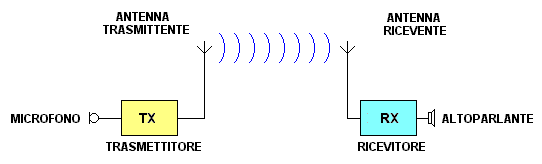
\includegraphics[width=0.8\textwidth]{Imgs/Radio}
\end{frame}

\begin{frame}{Propagazione delle onde elettromagnetiche}
	\framesubtitle{Antenna}
	La lunghezza di un'antenna è un parametro legato alla frequenza del segnale in uso, ciò significa che la \textbf{lunghezza dell'antenna determina quali frequenze essa può ricevere e trasmettere} nella maniera migliore e senza danneggiare il trasmettitore.\\
	\smallskip
	Generalmente la lunghezza di un'antenna può essere due o quattro volte inferiore alla lunghezza d'onda del segnale. Nel primo caso si dice che l'antenna è \textbf{mezz'onda}, nel secondo caso, che l'antenna è un \textbf{quarto d'onda}. Più la lunghezza dell'antenna si avvicina alla lunghezza d'onda, più l'antenna risulta efficiente e la portata migliorata.
	\begin{figure}
		\begin{columns}
			\hfill
			\column{.1\linewidth}
			\animategraphics[loop,width=2.5\textwidth]{10}{GifImages/Antenna/Antenna-}{0}{7}
			\column{.3\linewidth}
			%\caption{{\textcolor{gray!80}{[Immagine animata]}}}
			\qquad \tiny{\textcolor{gray!80}{[Immagine animata]}}
		\end{columns}
	\end{figure}
\end{frame}

\begin{frame}{Propagazione delle onde elettromagnetiche}
	\framesubtitle{Sistemi di propagazione delle onde elettromagnetiche}
	Le onde elettromagnetiche, una volta irradiate \textbf{dall'antenna trasmittente}, possono raggiungere \textbf{l'antenna ricevente} in quatto modi diversi:\\
	 \medskip
	 \begin{itemize}
	 	\item Onda terrestre o onda di superficie.
	 	\item Onda spaziale diretta.
	 	\item Onda spaziale riflessa dalla ionosfera.
	 	\item Onda spaziale riflessa dai satelliti.
	 \end{itemize}
 \medskip
 \centering
 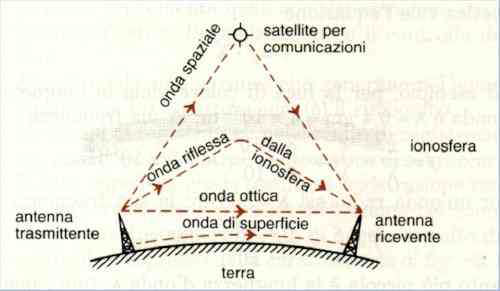
\includegraphics[width=0.35\textwidth]{Imgs/Propagazione}
	\end{frame}

\begin{frame}{Propagazione delle onde elettromagnetiche}
	\framesubtitle{Onda terrestre o onda di superficie}
	L'onda terrestre si ha quando le antenne {\vet Tx} e {\vet Rx} si trovano vicino al suolo, ad altezza relativamente piccola nei confronti della lunghezza d'onda della frequenza emittente ed entrambe le antenne sono polarizzate verticalmente.\\
	Questo tipo di onde si propaga rasente al suolo, seguendo al curvatura delle superficie terrestre.\\
	Il percorso che le onde possono compiere è essenzialmente limitato dall'assorbimanto di energia esercitato dal suolo, il quale in parte assorbe e riflette le onde che si propagano su di esso.\\
	L'attenuazione subita dalle onde è tanto maggiore quanto più è elevata la frequenza de segnale, pertanto, l'onda terrestre viene impiegata per la radiodiffusione ad onde lunghe e medie.\\	
\end{frame}

\begin{frame}{Propagazione delle onde elettromagnetiche}
		\framesubtitle{Onda spaziale diretta}
		L'onda spaziale diretta si ha quando le antenne {\vet Tx} e {\vet Rx} si trovano ad una altezza superiore rispetto alla lunghezza d'onda del segnale trasmesso.\\
		L'altezza sarà tale che le antenne si potranno considerare a \emph{"distanza ottica"}.\\
		Le onde dirette vengono solitamente impiegate per frequenze superiori si 30 MHz (detta \emph{Frequenza Critica}), cioè con lunghezza d'onda inferiore a dieci metri, quindi nelle trasmissioni televisive e radio FM.\\
		\medskip
		\centering
		 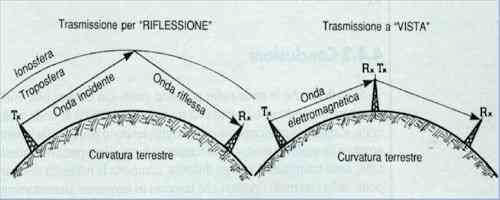
\includegraphics[width=0.5\textwidth]{Imgs/OndaDiretta}
\end{frame}

\begin{frame}{Propagazione delle onde elettromagnetiche}
	\framesubtitle{Frequenza critica}
	La frequenza critica è la massima frequenza per la quale la ionosfera è in grado di riflettere la radiazione elettromagnetica per incidenza verticale.\\
	\smallskip
	La \textbf{ionosfera} è una porzione dell'atmosfera dove la pressione dell'aria è così bassa che \textbf{elettroni} (di carica negativa) e \textbf{ioni} (di carica positiva) sono liberi di muoversi per un certo periodo senza cadere in prossimità di altre particelle ricombinandosi in atomi neutri.\\
	La causa primaria della \textbf{ionizzazione} di una porzione esterna dell'atmosfera è la \textbf{radiazione ultravioletta} generata dal sole.\\
	\smallskip
	Il livello di ionizzazione prodotta non varia uniformemente con la distanza della superficie terrestre, ma presenta un andamento regolare (ma non costante) all'interno di strati di differente spessore, all'incirca paralleli alla superficie terrestre, inoltre è caratterizzato da sensibili differenze tra uno strato e l'altro.\\ 
\end{frame}

\begin{frame}{Propagazione delle onde elettromagnetiche}
	\framesubtitle{Dimostrazione fisica della frequenza critica parte 1}
	Relazioni utili per l'analisi:\\
	\begin{itemize}
		\item Densità $ N $ degli elettroni per la ionosfera: $N = 1.24 \cdot 10^{4} \cdot f_{c(MHz)} cm^{-3}$
		\item $f = \sqrt{\frac{80.8 \cdot N \cdot (1+2\cdot\frac{h}{R})}{\sin^{2} \beta + 2\cdot\frac{h}{R}}}Hz$ 
		\item $MUF = f_{max}$
		\item $OTF = 0.85 \cdot MUF$
	\end{itemize}
\smallskip
Dove:\\
\begin{itemize}
	\item[] $N$ = Densità degli elettroni liberi.
	\item[] $f_c$ = Frequenza critica, ovvero la massima frequenza che viene riflessa per incidenza verticale dalla ionosfera.
	\item[] $f$ = Massima frequenza che viene riflessa da uno strato ionosferico di altezza $h$ e \\densità elettronica $N$, per un angolo di elevazione $\beta$.
	\item[] $R$ = Raggio terrestre = 6370 Km
	\item[] $h$ = Altezza dello strato ionico riflettente.
	\item[] $MUF$ = Maximum Usable Frequency.
	\item[] $OTF$ = Optimum Trafic Frequency. 
\end{itemize}
\end{frame}

\begin{frame}{Propagazione delle onde elettromagnetiche}
	\framesubtitle{Dimostrazione fisica della frequenza critica parte 2}
	La formula che fornisce la massima frequenza $f$ riflessa dalla ionosfera mostra che:\\
	\smallskip
	\begin{enumerate}
		\item A parità di angolo $\beta$ di elevazione e di altezza $h$ dello strato ionosferico, maggiore è la densità degli elettroni liberi (ovvero il grado di ionizzazione) e maggiore sarà la massima frequenza riflessa.
		\item A parità di condizioni ionosferiche (altezza $h$ e densità $N$), la massima frequenza utilizzabile è ottenuta quando l'angolo di elevazione $\beta$ è prossimo allo zero, ovvero quando si trasmette verso l'orrizzonte.
		\item Per angolo di elevazione $\beta$ uguali a novanta gradi, la massima frequenza diventa uguale alla frequenza critica $f_{c}$.
		\item la massima frequenza $f$ per angoli $\beta$ minori di novanta gradi è maggiore di $f_{c}$, ed \\aumenta fino al valore massimo per angolo $\beta$ uguale a zero gradi.
	\end{enumerate}
\end{frame}

\begin{frame}{Propagazione delle onde elettromagnetiche}
	\framesubtitle{Conclusione della dimostrazione fisica della frequenza critica }
	In conclusione:\\
	\smallskip
	Per un dato strato ionosferico, per stabilire un collegamento fra due punti, non è sufficiente che la frequenza scelta sia inferiore alla $MUF$, ma è anche necessario che essa sia pure maggiore della $LUF$ (Least Usable Frequency), nel senso che la frequenza deve essere "sufficientemente" alta da non subire un'attenuazione eccessiva da parte degli strati bassi.\\
	Pertanto la frequenza ideale di trasmissione, spesso coincidente con la $OTF$, deve soddisfare la relazione:\\
	\smallskip
	$LUF \leq f \leq MUF$
	\smallskip
	Infine, per date condizioni ionosferiche (densità $N$ ed altezza $h$), e per una data frequenza maggiore della frequenza critica $f_{c}$, l'angolo di radiazione (o elevazione) $\beta$ non deve superare un valore limite, detto angolo critico. In tal caso, la ionosfera non\\ produce riflessione ed il segnale va perso nell'atmosfera.
\end{frame}

\begin{frame}{Propagazione delle onde elettromagnetiche}
	\framesubtitle{Relazione tra la massima frequenza riflessa e l'angolo $\beta$}
	\centering
	 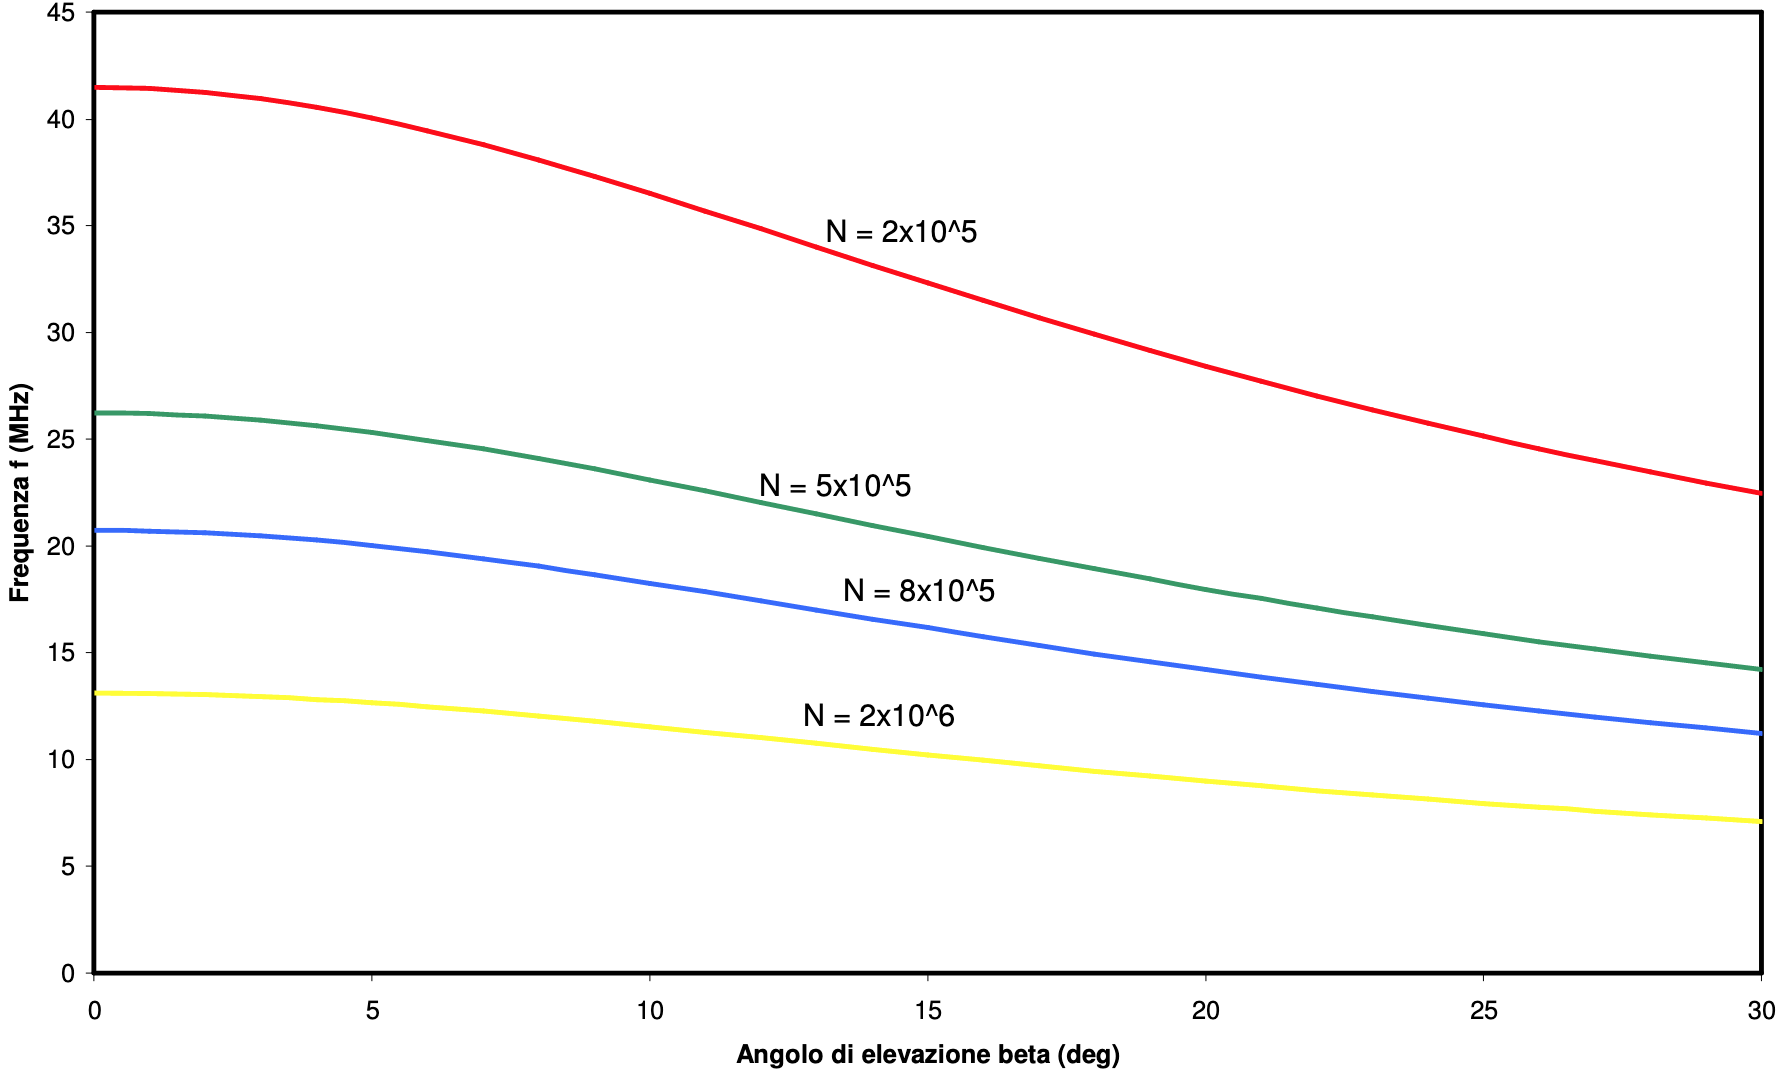
\includegraphics[width=0.7\textwidth]{Imgs/Beta}
\end{frame}

\begin{frame}{Propagazione delle onde elettromagnetiche}
	\framesubtitle{Onda spaziale riflessa dalla ionosfera}
	Le onde ionosferiche non raggiungono direttamente l'antenna {\vet Rx}, ma provengono "dall'alto" dopo essere state riflesse dalla ionosfera.\\
	La riflessione avviene perché queste onde hanno frequenza inferiore alla \emph{Frequenza Critica} di 30MHz.\\
	\medskip
	\centering
	 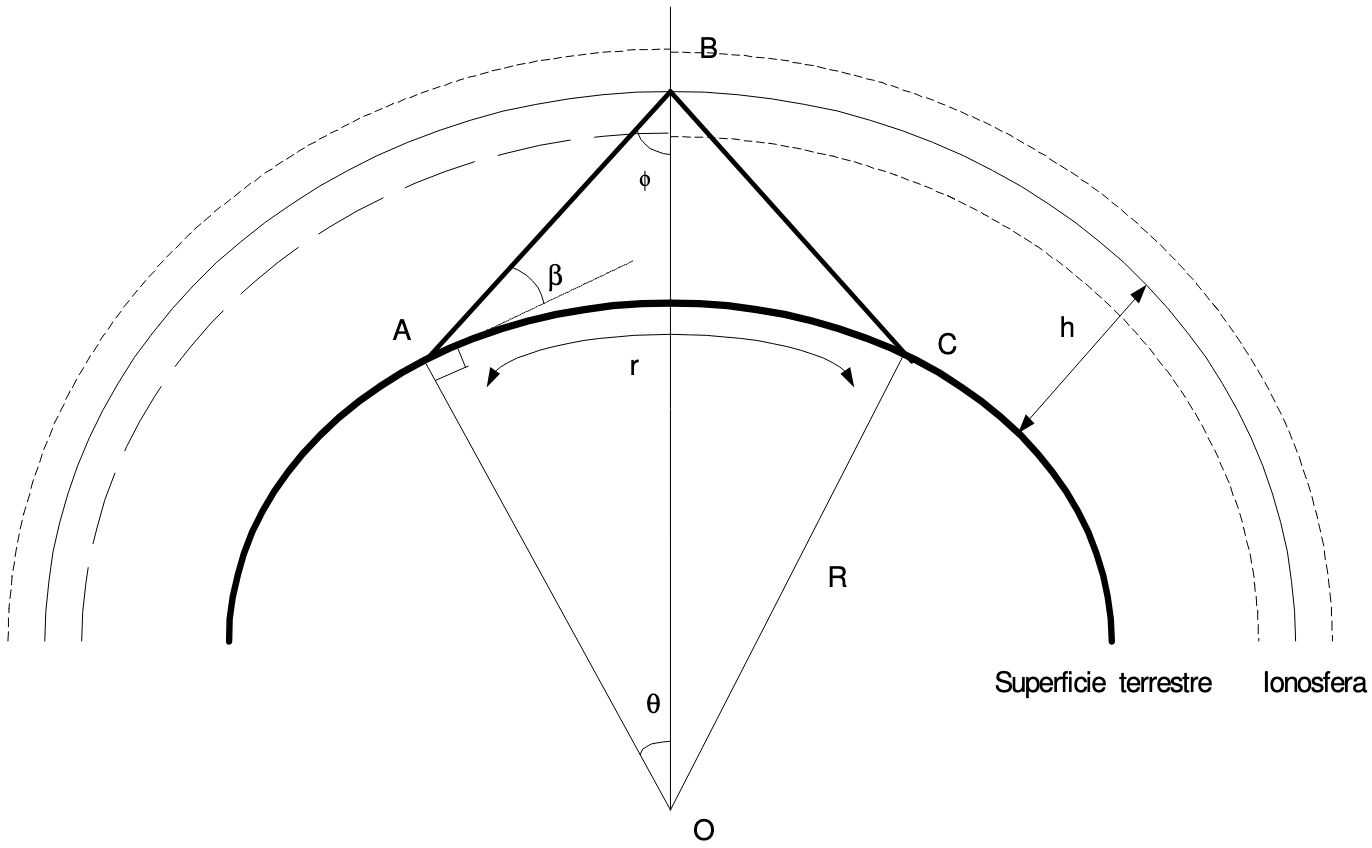
\includegraphics[width=0.45\textwidth]{Imgs/Ionosfera}
	\end{frame}

\begin{frame}{Propagazione delle onde elettromagnetiche}
	\framesubtitle{Onda spaziale riflessa dai satelliti}
	L'onda spaziale riflessa dai satelliti si ha quando un segnale viene inviato nello spazio con un angolo incidente molto piccolo ed indirizzato in un punto molto preciso dello spazio in cui è allocato un \emph{satellite geostazionario}.\\
	Il satellite, mantenendo rigorosamente costante la posizione nei confronti della Terra, si comporta come se fosse un'antenna di enorme altezza, capace di "riflettere" il segnale.\\
	Il satellite si comporta in effetti come antenne ricevente {\vet Rx} per i segnali che giungono da Terra e da antenna trasmittente {\vet Tx} per i segnali che da essa vengono poi irradiati verso Terra.\\
	\medskip
	\centering
	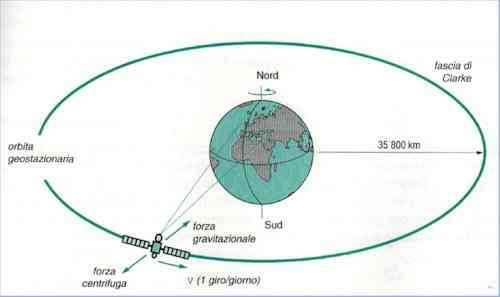
\includegraphics[width=0.35\textwidth]{Imgs/OndaSatellitare}
\end{frame}

\section{La banda nautica}
\begin{frame}
	\centering{{\textcolor{blue!80}{\huge{\textbf{La banda nautica}}}}}\\
\end{frame}

\begin{frame}{Frequenze nautiche}
	Le frequenze che rivestono maggiore importanza ed interesse per chi svolge operazioni in mare sono le frequenze in banda \textbf{VHF}.\\
	\smallskip
	Il range delle frequenze in base ad una spaziatura di 25 KHz è:\\
	\begin{itemize}
		\item Da 156.51 MHz (corrispondente al canale 1)
		\item A 162.025 MHz (corrispondente al canale 88)
	\end{itemize}
\smallskip
Si tratta di onde che si propagano a \textbf{distanza ottica}, ciò significa che la presenza di \textbf{ostacoli} o la \textbf{curvatura terrestre} ne impediscono la \textbf{diffusione}, se non tramite dispositivi di ripetizione del segnale.\\
\end{frame}

\section{I canali VHF}
\begin{frame}
	\centering{{\textcolor{blue!80}{\huge{\textbf{I canali VHF}}}}}\\
\end{frame}

\begin{frame}{I canali VHF marini}
	\framesubtitle{Introduzione}
	Il \textbf{Piano Nazionale per la Ripartizione delle Frequenze} (PNRF) costituisce un vero e proprio \emph{piano regolatore dell'utilizzo dello spettro radioelettrico} in Italia.\\
	\smallskip
	Lo scopo del piano è quello di stabilire, in ambito nazionale e per il tempo di pace:
	\begin{itemize}
		\item \textbf{L'attribuzione} ai diversi servizi delle bande di frequenza.
		\item Indicare per ciascun servizio, nell'ambito delle singole bande, \textbf{l'autorità governativa preposta} alla gestione delle frequenze.
		\item Indicare le principali \textbf{utilizzazioni} civili e verificare l'efficiente utilizzo dello spettro, al fine di \textbf{liberare risorse}
	\end{itemize}
\end{frame}

\begin{frame}{I canali VHF marini}
	\framesubtitle{Tipologia dei canali VHF marini}
	Molti dei canali VHF sono detti \textbf{duplex} e sono quelli che hanno una frequenza di trasmissione {\vet Tx} diversa da quella ricezione {\vet Rx}.\\
	Quelli che invece usano la stessa frequenza per trasmettere e ricevere sono detti \textbf{simplex}.\\
	\smallskip
	I canali \textbf{duplex} danno la possibilità a chi è dotato di un apparato VHF professionale con questa funzionalità, di poter trasmettere e ricevere simultaneamente.\\
	\medskip
	\centering
	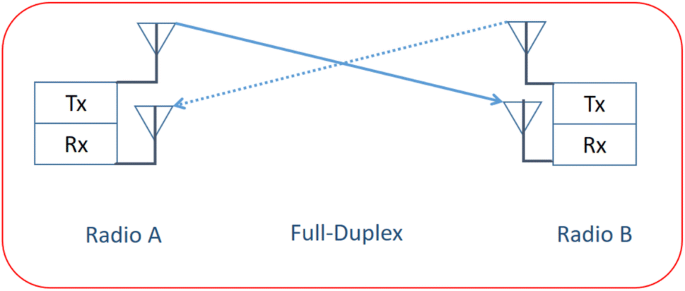
\includegraphics[width=0.5\textwidth]{Imgs/Duplex}
\end{frame}

\begin{frame}{Tabella Canali VHF marini}
	\begin{columns}
		\column{.45\linewidth}
		\resizebox{1\textwidth}{!}{
			\begin{tabular}{|l|l|l|l|l|}
			\hline
			N.Canale & Freq. Tx & Freq. Rx & Uso & Simplex \\ \hline
			1 & 156.050 & 160.650 & Corrispondenza pubblica e operazioni portuali &\\ \hline
			2 & 156.100 & 160.700 & Corrispondenza pubblica e operazioni portuali &\\ \hline
			3 & 156.150 & 160.750 & Corrispondenza pubblica e operazioni portuali &\\ \hline
			4 & 156.200 & 160.800 & Corrispondenza pubblica e operazioni portuali &\\ \hline
			5 & 156.250 & 160.850 & Corrispondenza pubblica e operazioni portuali &\\ \hline
			6 & 156.300 & 156.300 & Sicurezza nave-nave & X \\ \hline
			7 & 156.350 & 160.950 & Corrispondenza pubblica e operazioni portuali &\\ \hline
			8 & 156.400 & 156.400 & Commerciale nave - nave & X \\ \hline
			9 & 156.450 & 156.450 & Commerciale & X \\ \hline
			10 & 156.500 & 156.500 & Commerciale & X \\ \hline
			11 & 156.550 & 156.550 & Commerciale & X \\ \hline
			12 & 156.600 & 156.600 & Operazioni portuali & X \\ \hline
			13 & 156.650 & 156.650 & Sicurezza nave-nave in navigazione & X \\ \hline
			14 & 156.700 & 156.700 & Operazioni portuali & X \\ \hline
			15 & 156.750 & 156.750 & Operazioni portuali - Solo Bassa Potenza & X \\ \hline
			16 & 156.800 & 156.800 & Chiamata e soccorso internazionale & X \\ \hline
			17 & 156.850 & 156.850 & Operazioni portuali - Solo Bassa Potenza & X \\ \hline
			18 & 156.900 & 161.500 & Operazioni portuali &\\ \hline
			19 & 156.950 & 161.550 & Operazioni portuali &\\ \hline
			20 & 157.000 & 161.600 & Operazioni portuali &\\ \hline
			21 & 157.050 & 161.650 & Operazioni portuali &\\ \hline
			22 & 157.100 & 161.700 & Operazioni portuali &\\ \hline
			23 & 157.150 & 161.750 & Corrispondenza pubblica &\\ \hline
			24 & 157.200 & 161.800 & Corrispondenza pubblica &\\ \hline
			25 & 157.250 & 161.850 & Corrispondenza pubblica &\\ \hline
			26 & 157.300 & 161.900 & Corrispondenza pubblica &\\ \hline
			27 & 157.350 & 161.950 & Corrispondenza pubblica &\\ \hline
			28 & 157.400 & 162.000 & Corrispondenza pubblica &\\ \hline
			60 & 156.025 & 160.625 & Corrispondenza pubblica &\\ \hline
		\end{tabular}}
		\column{.45\linewidth}
		\resizebox{1\textwidth}{!}{
			\begin{tabular}{|l|l|l|l|l|}
			\hline
			N.Canale & Freq. Tx & Freq. Rx & Uso & Simplex \\ \hline
		61 & 156.075 & 160.675 & Corrispondenza pubblica &\\ \hline
		62 & 156.125 & 160.725 & Corrispondenza pubblica &\\ \hline
		63 & 156.175 & 160.775 & Corrispondenza pubblica &\\ \hline
		64 & 156.225 & 160.825 & Corrispondenza pubblica &\\ \hline
		65 & 156.275 & 160.875 & Corrispondenza pubblica &\\ \hline
		66 & 156.325 & 160.925 & Corrispondenza pubblica &\\ \hline
		67 & 156.375 & 156.375 & Nave - nave + Operazioni Portuali & X \\ \hline
		68 & 156.425 & 156.425 & Bollettino Nautico - Operazioni Portuali  & X \\ \hline
		69 & 156.475 & 156.475 & Nave - Nave in Operazioni portuali & X \\ \hline
		70 & 156.525 & 156.525 & Riservato al DSC & X \\ \hline
		71 & 156.575 & 156.575 & Nave - nave + Operazioni Portuali & X \\ \hline
		72 & 156.625 & 156.625 & Nave - nave + Nave - Velivolo & X \\ \hline
		73 & 156.675 & 156.675 & Nave - nave + Nave - Velivolo & X \\ \hline
		74 & 156.725 & 156.725 & Operazioni portuali & X \\ \hline
		75 & 156.775 & 156.775 & Nave - Nave in porto - Solo Bassa Potenza & X \\ \hline
		76 & 156.825 & 156.825 & Nave - Nave in porto - Solo Bassa Potenza & X \\ \hline
		77 & 156.875 & 156.875 & nave - nave & X \\ \hline
		78 & 156.925 & 161.525 & Corrispondenza pubblica + Operazioni Portuali &\\ \hline
		79 & 156.975 & 161.575 & Operazioni portuali &\\ \hline
		80 & 157.025 & 161.625 & Operazioni portuali &\\ \hline
		81 & 157.075 & 161.675 & Corrispondenza pubblica + Operazioni Portuali &\\ \hline
		82 & 157.125 & 161.725 & Corrispondenza pubblica + Operazioni Portuali &\\ \hline
		83 & 157.175 & 161.775 & Corrispondenza pubblica &\\ \hline
		84 & 157.225 & 161.825 & Corrispondenza pubblica &\\ \hline
		85 & 157.275 & 161.875 & Corrispondenza pubblica &\\ \hline
		86 & 157.325 & 161.925 & Corrispondenza pubblica &\\ \hline
		87 & 157.375 & 157.375 & Corrispondenza pubblica & X \\ \hline
		88 & 157.425 & 157.425 & Corrispondenza pubblica & X \\ \hline
	\end{tabular}}
	\end{columns}
\end{frame}

\section{L'alfabeto internazionale}
\begin{frame}
	\centering{{\textcolor{blue!80}{\huge{\textbf{L'alfabeto internazionale}}}}}\\
\end{frame}

\begin{frame}{Alfabeto fonetico NATO}
	\framesubtitle{Introduzione}
	\textbf{L'alfabeto fonetico telegrafico}, chiamato spesso anche \textbf{alfabeto fonetico NATO}, venne sviluppato negli anni cinquanta dall'Organizzazione Internazionale dell'Aviazione Civile (\textbf{ICAO}) per essere comprensibile (e pronunciabile) per tutti i piloti e gli operatori dell'aviazione civile.\\
	Il suo utilizzo è prescritto dagli standard fraseologici aeronautici internazionali.\\
	Questo codice è oggi utilizzato anche nelle \textbf{trasmissioni Terra-Bordo-Terra} in ambito navale allo scopo di evitare fraintendimenti tra chi trasmette e chi riceve.\\
\end{frame}

\begin{frame}{Alfabeto fonetico NATO}
	\framesubtitle{Tabella lettere dell'alfabeto fonetico NATO}
	
		\begin{columns}
			\hfill
		\column{.3\linewidth}
			\begin{tabular}{|l|l|}
			\hline
			\textbf{A} - Alpha & \textbf{N} - November \\ \hline
			\textbf{B} - Bravo & \textbf{O} - Oscar \\ \hline
			\textbf{C} - Charlie & \textbf{P} - Papa \\ \hline
			\textbf{D} - Delta & \textbf{Q} - Quebec \\ \hline
			\textbf{E} - Echo & \textbf{R} - Romeo \\ \hline
			\textbf{F} - Foxtrot & \textbf{S} - Sierra \\ \hline
			\textbf{G} - Golf & \textbf{T} - Tango \\ \hline
			\textbf{H} - Hotel & \textbf{U} - Uniform \\ \hline
			\textbf{I} - India & \textbf{V} - Victor \\ \hline
			\textbf{J} - Juliet & \textbf{W} - Whiskey \\ \hline
			\textbf{K} - Kilo & \textbf{X} - Xray \\ \hline
			\textbf{L} - Lima & \textbf{Y} - Yankee \\ \hline
			\textbf{M} - Mike & \textbf{Z} - Zulu \\ \hline
		\end{tabular}
		\column{.5\linewidth}
		Esempio: volendo fare lo spelling del nominativo dell'imbarcazione “SIBILLA”, si dirà: \emph{“ Sierra, India, Bravo, India, Lima, Lima, Alfa”}.
	\end{columns}
\end{frame}

\begin{frame}{Alfabeto fonetico NATO}
	\framesubtitle{Numeri dell'alfabeto fonetico NATO}
	I numeri devono essere trasmessi \textbf{Pronunciando le cifre separatemene tranne le migliaia intere}.\\
	I multipli interi di mille devono essere trasmessi pronunciando ogni cifra delle migliaia seguite dalla parola “Mille”.\\
	I decimali saranno preceduti dalla parola punto (o decimale).\\
	\smallskip
	Chi riceve, potrà richiedere la ripetizione dei numeri in modo tale da poterli convalidare.\\
\end{frame}

\begin{frame}{Alfabeto fonetico NATO}
	\framesubtitle{Esempi di pronuncia dei numeri dell'alfabeto fonetico NATO}
		\begin{itemize}
		\item 10 \qquad (Uno Zero)
		\item 97 \qquad (Nove Sette)
		\item 721 \qquad (Sette Due Uno)
		\item 100 \qquad (Mille)
		\item 1300 \qquad (Uno Tre Zero Zero)
		\item 10000 \qquad (Uno Zero Mille)
		\item 122.6 \qquad (Uno Due Due punto Sei)
	\end{itemize}
\end{frame}

\section{La classificazione dei messaggi}
\begin{frame}
	\centering{{\textcolor{blue!80}{\huge{\textbf{La classificazione dei messaggi}}}}}\\
\end{frame}

\begin{frame}{Ordine di priorità dei messaggi}
	I messaggi radiotelegrafici hanno una scala di priorità ovvero un diritto di precedenza ben definito:\\
	\medskip
	\begin{enumerate}
		\item \textbf{Soccorso} - Lanciato da chiunque si trovi in stato di pericolo o voglia prestare soccorso.
		\item \textbf{Urgenza} - Concerne la sicurezza di chiunque si trovi in seria difficoltà ma non corra un pericolo immediato.
		\item \textbf{Sicurezza} - Lanciato da chiunque voglia segnalare un pericolo per la navigazione
	\end{enumerate}
\medskip
Il \textbf{canale 16} (156.8 MHz) è il canale preposto per il lanciare questo tipo di messaggi, il quale, \textbf{non deve essere utilizzato nei primi tre minuti di ogni mezz'ora}, in modo da lasciare il canale libero per l'ascolto di eventuali chiamate di soccorso. Nel tempo rimanente, deve \\essere utilizzato solo per motivi tecnici.
\end{frame}

\begin{frame}{Messaggio di soccorso}
	\framesubtitle{Stato di pericolo}
	
	Nello\textbf{stato di pericolo} il messaggio sarà preceduto tre volte dalla parola \textbf{MAYDAY} pronunciato alla francese \emph{“medé”}, seguito tre volte dal nominativo dell'unità che richiede immediata assistenza.\\
	Il testo del messaggio deve contenere indicazioni non ambigue affinché risulti agevole, a chi lo riceve, localizzare l'unità in pericolo attraverso la dichiarazione della posizione, dell'ora, della velocità e della rotta.\\
	Il Comandante dell'unità che richiede immediata assistenza è bene che dichiari inoltre la natura del pericolo e le proprie intenzioni.\\
	\medskip
	{\textcolor{red!80}{Le Unità non coinvolte nelle operazioni di soccorso dovranno mantenere il più assoluto\\ \textbf{silenzio radio}.}}
\end{frame}


\begin{frame}{Messaggio di soccorso}
	\framesubtitle{Prestare soccorso}
	Nel caso che si voglia \textbf{prestare soccorso}, rilanciando il messaggio di una imbarcazione in \textbf{stato di pericolo} al quale non è stata percepita una risposta, il Comandante che riceve la richiesta, dopo aver dato il \emph{"ricevuto"} alla nave in stato di pericolo, rilancerà il messaggio a una stazione a terra (che possa assicurare assistenza)  facendo precedere la comunicazione dalle parole \textbf{MAYDAY RELÈ}, (pronunciate alla francese \emph{“medé relé”}), ripetuta tre volte.\\
	\medskip
	{\textcolor{red!80}{Le Unità non coinvolte nelle operazioni di soccorso dovranno mantenere il più assoluto \textbf{silenzio radio}.}}
\end{frame}

\begin{frame}{Messaggi di urgenza}
	I messaggi di \textbf{urgenza} si riferiscono alla \textbf{sicurezza} di chiunque si trovi in seria difficoltà ma non corra un pericolo immediato.\\
	\smallskip
	Nello stato di \textbf{urgenza} il messaggio sarà preceduto tre volte dalla parola \textbf{PAN} ripetuta tre volte e seguita tre volte dal nominativo dell'Unità che fa la richiesta.\\
	\medskip
	I messaggi di urgenza si usano ad esempio per comunicare che: un passeggero imbarcato che sta male, un guasto al motore, una perdita di combustibile... etc.
\end{frame}

\begin{frame}{Messaggi inerenti alla sicurezza}
Un messaggio \textbf{inerente alla sicurezza} identifica un \textbf{pericolo per la navigazione}. La parola per effettuare una chiamata di \textbf{sicurezza} è \textbf{SECURITÉ}.\\
\smallskip
Anche in questo caso il messaggio inerente alla sicurezza sarà preceduto dalla parola \textbf{SECURITÉ} ripetuta tre volte, seguita dal messaggio di Sicurezza per la Navigazione ed eventualmente dalla posizione del pericolo.
\end{frame}

\section{Trasmissione e ricezione}
\begin{frame}
	\centering{{\textcolor{blue!80}{\huge{\textbf{Trasmissione e ricezione}}}}}\\
\end{frame}

\begin{frame}{Buone pratiche per l'uso del VHF di bordo}
	Delle buone pratiche da seguire per il corretto utilizzo del VHF di bordo sono:\\
	\begin{itemize}
		\item Regolare opportunamente le impostazioni ed i volumi della radio in modo che i messaggi vengano compresi con chiarezza.
		\item Prima di trasmettere un messaggio, bisogna aver ben chiaro in mente cosa si vuole comunicare,\textbf{evitando di trasmettere continue correzioni o ripetizioni}.
		\item Per quanto possibile, i messaggi devono essere \textbf{brevi e concisi}.
		\item Rendersi conto del \textbf{“contesto-radio”} in cui ci si trova ascoltando anche i messaggi altrui per evitare di interromperli, tenendo presente che la normale procedura di comunicazione prevede una richiesta ed un risposta.
		\item Si devono \textbf{evitare in modo assoluto considerazioni e chiacchiere personali}.
		\item {\textcolor{red!80}{Essendo il canale uno spazio pubblico, la professionalità dell'operatore è sotto gli \\occhi di tutti!}}
	\end{itemize}
\end{frame}

\begin{frame}{Operatività sul canale 16}
	Il canale 16 dei VHF marini viene utilizzato per effettuare una \textbf{segnalazioni di soccorso, d'emergenza e di sicurezza}, pertanto non deve essere utilizzato per qualsiasi altro tipo di comunicazione.\\
	\smallskip
	Prima di \textbf{trasmettere} un messaggio, è necessario assicurarsi che sul canale non ci siano altre comunicazioni d'emergenza attive in attesa di essere trasferite su un altro canale, (spesso suggerito dalla Guardia Costiera).\\
	\smallskip
	Nei \textbf{ primi tre minuti di ogni mezz'ora} va mantenuto su questo canale il \textbf{silenzio radio} ed ogni messaggio trasmesso deve essere breve e conciso,  in modo da privilegiare le comunicazioni d'emergenza, tenendo il canale il più libero possibile.
\end{frame}

\begin{frame}{Utilizzo del VHF}
	\framesubtitle{Potenza di un apparato VHF}
	L'intensità del segnale di un apparato VHF dipende dalla potenza di trasmissione e dall'efficenza dell'antenna installata.\\
	\smallskip
	In media una \textbf{radio VHF portatile} possiede una portata di \textbf{circa nove miglia}, per una potenza di trasmissione compresa \textbf{tra i tre ed i cinque Watt}.\\
	Invece una \textbf{radio VHF fissa} possiede una portata di \textbf{circa quattordici miglia}, per una potenza di trasmissione di \textbf{venticinque Watt}.\\
	\smallskip
	In entrambi i modelli è possibile scendere di un Watt (con un apposito pulsante) per comunicazioni a corto raggio, in modo da non invadere l'eterere a distanze inutili con la possibilità di creare interferenze ad altre comunicazioni. \\
	Mentre se si deve trasmettere a lunga distanza si sfrutta la potenza massima.\\
\end{frame}

\begin{frame}{Utilizzo del VHF}
	\framesubtitle{Esempio di apparati ricetrasmittenti VHF}
	\begin{figure}
		\begin{columns}
			\column{.3\linewidth}
			 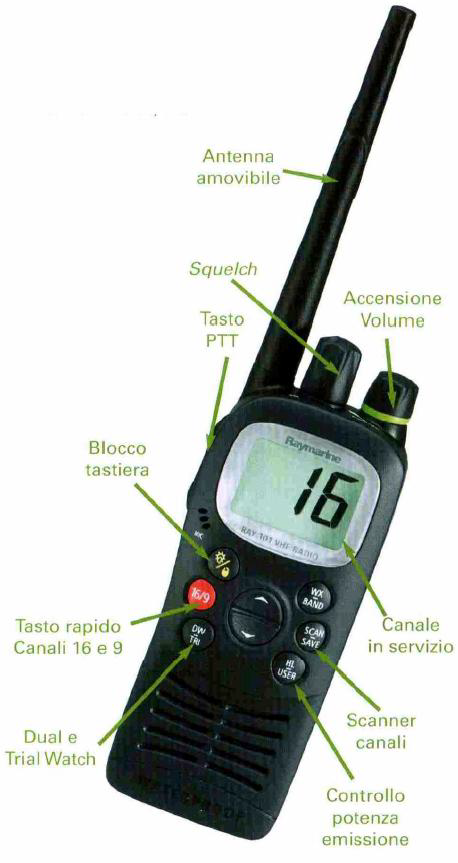
\includegraphics[width=0.7\textwidth]{Imgs/VHFPort}
			\column{.35\linewidth}
			 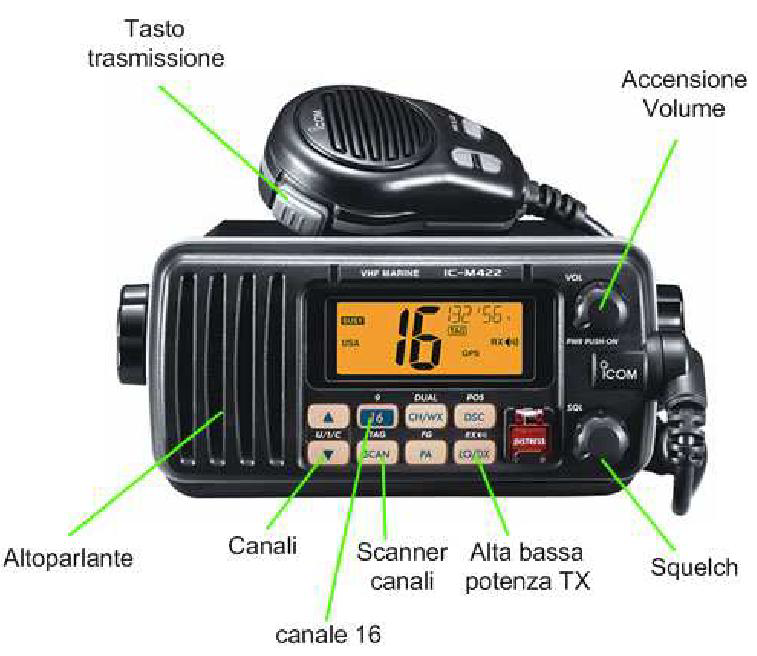
\includegraphics[width=1\textwidth]{Imgs/VHFFis}
		\end{columns}
	\end{figure}
\end{frame}

\begin{frame}{Effettuare una chiamata}
	Per effettuare una chiamata si \textbf{sintonizza} l'apparato VHF su un canale noto al ricevente della trasmissione, accertandosi che non ci siamo altre comunicazioni in corso sullo stesso canale.\\
	\smallskip
	Quindi si procede alla trasmissione chiamando \textbf{per tre volte il nominativo della stazione}, preceduto dalla parola "qui". Normalmente il nominativo della stazione da contattare è il nome dell'unità.\\
	\medskip
	\textbf{Per esempio:}\\
	\emph{Papa Charlie Uno Zero Tre Cinque - Papa Charlie Uno Zero Tre Cinque - Papa Charlie Uno Zero Tre Cinque, qui Papa Charlie Uno Zero Tre Tre}\\
	\smallskip
	Se "Papa Charlie Uno Zero Tre Cinque" non dovesse rispondere si attende per due minuti e poi si effettua di nuovo la chiamata.
\end{frame}

\begin{frame}{Rispondere a una chiamata}
I canali VHF più usati sono \emph{simplex}, per cui la trasmissione e la ricezione avvengono sulla stessa frequenza, quindi non si può parlare e ascoltare contemporaneamente.
\smallskip
Al fine di agevolare le comunicazioni,  il dialogo due operatori deve essere scandito da una serie di parole codificate: si usa \textbf{"passo"} o \textbf{"cambio"} per indicare che si passa dalla fase di trasmissione a quella di ricezione e \textbf{"ricevuto"} per indicare che si è compreso il messaggio.\\
Per segnalare la fine della trasmissione si usa la frase: \textbf{"passo e chiudo"}.\\
\smallskip
È inoltre opportuno segnalare la \textbf{scala di comprensibilità dei messaggi}:\\
\begin{enumerate}
	\item Incomprensibile.
	\item Comprensibile a tratti.
	\item Comprensibile ma con difficoltà.
	\item Comprensibile.
	\item Perfettamente comprensibile.
\end{enumerate}
\smallskip
\emph{Un tempo, essendo la scala scandita in quinti, si diceva "ricevo un quinto"(quindi la \\portante), oggi è preferibile dire: \textbf{"ricevo uno"} oppure \textbf{"ricevo forza uno"}.}
\end{frame}

\begin{frame}{Il canale 68}
	Il canale 68 è il canale preposto per la trasmissione del \textbf{Bollettino del Mare} relativo ai bacini del \textbf{Mediterraneo}. La trasmissione è emessa \textbf{24 ore su 24} dall'\textbf{Istituto Idrografico della Marina Militare}.
	\smallskip
	La previsione è valida 12 ore e viene rinnovata ogni 6 ore. Il rinnovi vengono effettuati intorno alle ore 00 - 06 - 12 -18.\\
	\smallskip
	Il bollettino del mare (anche detto \textbf{Meteomar}) comprende:
	\begin{itemize}
		\item Avvisi di burrasche in corso o previste.
		\item Avvisi di temporali in corso o previsti.
		\item Analisi della situazione.
		\item Situazione e tendenza della forza dei mari e dei venti per le ore successive
		\item Avvisi ai naviganti di primaria importanza.
	\end{itemize}
\end{frame}

\begin{frame}{Norme per l'utilizzo del VHF}
	Tutte le unità che navigano oltre le \textbf{sei miglia} dalla costa deve essere presente un dispositivo ricetrasmittente VHF (di tipo fisso o portatile), mentre nelle unità di \textbf{lunghezza} superiore a \textbf{24 metri} deve essere installato \textbf{obbligatoriamente} un apparato VHF di tipo \textbf{fisso}.\\
	Entro le sei miglia dalla costa l'uso del VHF è facoltativo.\\
	\medskip
	{\textcolor{red!80}{L'apparato VHF,\textbf{con tale documentazione}, va usato solo ai fini della sicurezza, con esclusione tassativa dell'effettuazione di traffico di corrispondenza pubblica.}}
\end{frame}

\begin{frame}{Certificato limitato di radiotelefonista}
	Il certificato limitato di radiotelefonista è una certificazione necessaria per l'utilizzo di apparecchiature ricetrasmittenti VHF a bordo di imbarcazioni o navi; essa è regolata dall'\textbf{art. 165 del Codice di comunicazioni elettroniche}.\\
	\medskip
	Questo certificato è disponibile in due tipologie:
	\begin{enumerate}
		\item Per impianti con potenza fino a 60 watt su navi di stazza lorda inferiore alle 150 tonnellate (ottenibile senza sostenere esami).
		\item Per ogni tipo di impianto installato su navi di stazza lorda inferiore a 1600 tonnellate (rilasciato dopo il superamento di un esame).
	\end{enumerate}
\smallskip
Entrambi i certificati vengono emessi dalle sedi regionali del \textbf{Ministero delle \\Comunicazioni}.
\end{frame}

\begin{frame}{Radio ad uso impresa (Approfondimento)}
	Per ottenere la licenza per stazioni radio (es. radio taxi, servizi di vigilanza, associazioni per la protezione civile), sia fisse che mobili, bisogna inviare la modulistica indicata dall'\textbf{art. 107 del Decreto legislativo 259/03}, cioè \textbf{allegato 14, allegato 15 e allegato 16} presso:\\
	\medskip
	Ministero dello Sviluppo Economico - Comunicazioni\\
	Direzione Generale per i servizi di comunicazione elettronica e di radiodiffusione – Divisione II\\
	Viale America, 201 - 00144 Roma\\
	\medskip
	L'ufficio competente, dopo avere effettuato \textbf{un'istruttoria tecnica e amministrativa}, comunicherà l'entità del contributo e i dati per effettuare il versamento in questione.
\end{frame}

\begin{frame}{Sanzioni (Approfondimento)}
	\begin{itemize}
		\item Art. 102 Codice delle Comunicazioni Elettroniche (installazione ed esercizio di comunicazione elettronica senza autorizzazione) - sanzione da 300€ a 10000€
		\item Art. 172 Codice delle Comunicazioni Elettroniche ( fare uso a bordo di unità nautiche di apparecchiature radio nelle bande del servizio mobile marittimo in assenza di autorizzazione) - sanzione da 120€ a 485€
		\item Art. 1200 Codice della Navigazione (abusivo trasporto o impiego di apparecchi radiotrasmittenti a bordo di unità nautiche) - sanzione da 1032€ a 6197€
		\item Art. 217 Codice delle comunicazioni Elettroniche (uso indebito del segnale di soccorso) - arresto sino a 6 mesi o ammenda sino a 670€
		\item Art. 658 Codice Penale (procurato allarme presso l’autorità) - arresto sino a 6 mesi o ammenda da 10€ a 516€
	\end{itemize}
\end{frame}

\addtocontents{toc}{\protect\setcounter{tocdepth}{0}}
\section{Indice}
\begin{frame}[label = index]
	%\index{generate}
	\tableofcontents
\end{frame}

\end{document}
